\chapter{Evaluation}

After full implementation of the design proposed to the project, there has to be careful evaluation of the outcomes, or more specifically improvements introduced by such an implementation. At this point the distributed version with built-in clustering is fully developed, and the focus is on the possible criteria of the resulting product evaluation.

\section{Current Solutions}

There are already quite a few projects within the area of distributed neural network simulation. Here are some that are most similar in structure with the current project (most of them were mentioned in the Background section).

\subsection{Blue Brain Project}

The Blue Brain Project initiated in collaboration by IBM and EPFL, is aimed to reconstruct the virtual brain on the BlueGene/L supercomputer.\cite{BlueBrain} This project set its objectives in simulating the real virtual brain, as it has already succeded the simulation of a rat cortex. With the sheer numbers of neurons present in simulation closing to $10^9$, this is the project with the most resource power among listed here.

\subsection{SpikeNET}

The SpikeNET simulator focuses on the scalability of the simulation - it is concentrated on simulation of large number of integrate-and-fire neurons which spikes are computed in parallel\cite{ArnaudDelorme1999}. For most parts of its implementation SpikeNET is quite similar to the NeMo project. However, its parallel computation implementation does not exploit a fully distributed parallelism, i.e. most of computation still lies within the scope of one process.

\subsection{OpenSim}

The OpenSim project on the other hand, relies on distribution of neural simulation into a set of parallelizable sub-tasks across a cluster of machines\cite{OpenSim}. However, due to the age of its most recent implementation, the techniques used within it might already be outdated, as more efficient communication channels were developed. Nevertheless, OpenSim, due to the fact that it relies on a fully distributed system, has many similarities in structure with this project. \\ \\


Even though, all of these projects could be compared against the MPI NeMo, the differences between the implementations alone will not be sufficient to make a fully informed judgement. The problem is the lack of common ground - all of these implementations vary in the ways of neuron representation, SpikeNET lacks delay functionality and Blue Brain is built on the platform which resource base cannot be challenged by the resources of NeMo project.

Therefore, a much more sensible approach would be to compare the current version of distributed system against the "clean" NeMo version and see which particular points of simulation are different between those two.

\clearpage

\section{Criteria of Comparison}

As the test platforms are chosen, it is time to pick a set of criterias which will tested to produce informative results. In order to pick the most informative criteria, there has to be an insight into the main variables within simulation. Those are:

\begin{itemize}
\item{\textbf{Setup Time}}

This criteria comprises the temporal requirements for the simulation to be set up in order to be run. Within core NeMo functionality, this time would be comprised of the simulation setup time which is almost negligible, since the Network object constructed, operates within Simulation. For the distributed system, however, startup time is split differently: it includes the clustering time and initialisation parameters distribution window - which could be further split into 4 steps - mapper, configuration, neurons and synapses.

\item{\textbf{Simulation Time}}

The simulation time is a measure of the simulator performance according to the time spent on the actual simulation; the variables that are set for the simulations are:

\begin{enumerate}	
	\item{Number of neurons} within the network
	\item{Number of synapses per neuron}
	\item{Number of simulation steps} - constraint put on the number of simulation steps to derive time requirement per step.
\end{enumerate}

Therefore, by iterating through each of these variables, while keeping others constant, it is possible to get the dependency of the current implementation on the particular parameter, and how its value affects the overall simulation.

\item{\textbf{Network throughput}}

Last criteria that could also represent the network - total spiking within network during simulation. This value highly depends on the number of neurons and the overall interconnectivity - the current implementation would only show the number of fired neurons and external spike deliveries.

\end{itemize}

Having set out all of the meaningful criteria, it is time to look at them in detail and compare the data gathered with different systems.

\section{Setup Time}

This section will cover the simulation setup stage of the distributed system's initialisation.

\subsubsection{MPI clustering and distribution overhead}

\begin{figure}[h]
\begin{center}
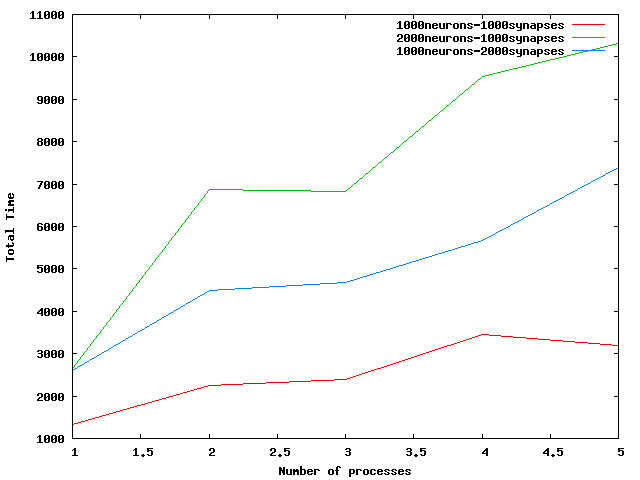
\includegraphics[scale = 0.5]{images/setup_comparison.png}
\end{center}
\caption{Comparison of setup time to the number of neurons, synapses and processes}
\end{figure}

From the above graph it is easily observable that the most amplifying factor for simulation setup time is the number of neurons. The setup time, however, can be further split into the 5 times - clustering, mapper, configuration, neuronal and synaptic distributions.

The ones having the most effect on the simulation setup time are clustering and synaptic distribution. Now, if those are observed closer under particular circumstances, their dependance upon other variables is clearly seen:

\begin{figure}[ht]
\begin{minipage}[b]{0.5\linewidth}
\centering
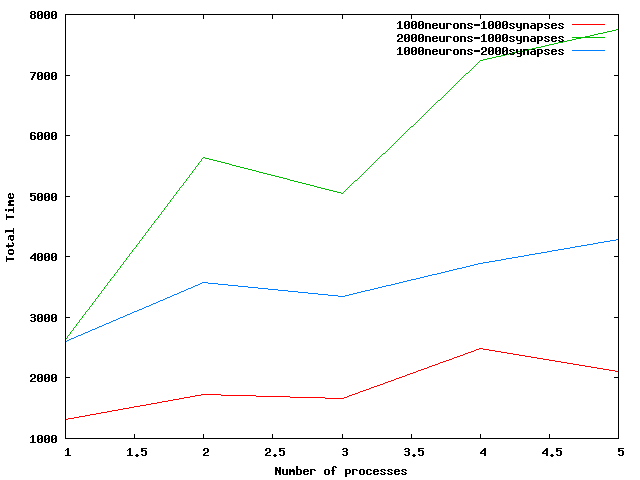
\includegraphics[width=\textwidth]{images/syndistr.png}
\caption{Synaptic distribution}
\label{fig:figure1}
\end{minipage}
\hspace{0.5cm}
\begin{minipage}[b]{0.5\linewidth}
\centering
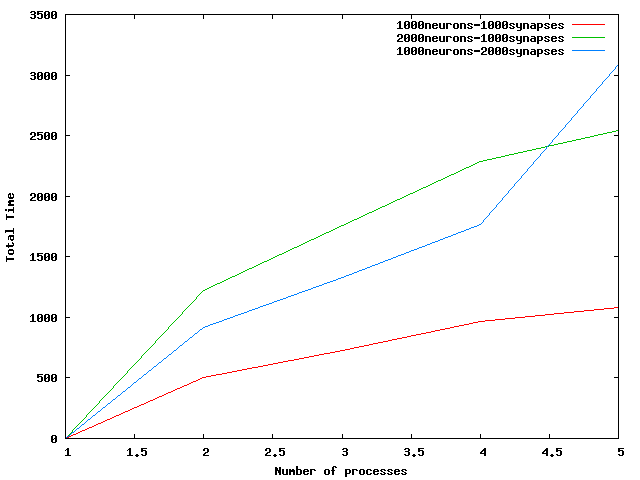
\includegraphics[width=\textwidth]{images/cluster.png}
\caption{Clustering}
\label{fig:figure2}
\end{minipage}
\end{figure}

From these graphs, it can be concluded that synaptic distribution depends more on the number of neurons and workers rather than on the per-neuron synapse count. As for the clustering, its timeline correlates with the increase in the number of processes - which is logically correct, since this means more calls to the clustering function at the startup.

\section{Simulation Time}

This section attempts evaluate the collected results of running multiple distributed simulations against the original NeMo simulation, and show the particular differences through simulation running time. The results of this evaluation show that even though the system has been implemented, there is still much more work on its optimisation.

\subsection{Number of neurons}

\begin{figure}[h!]
\begin{center}
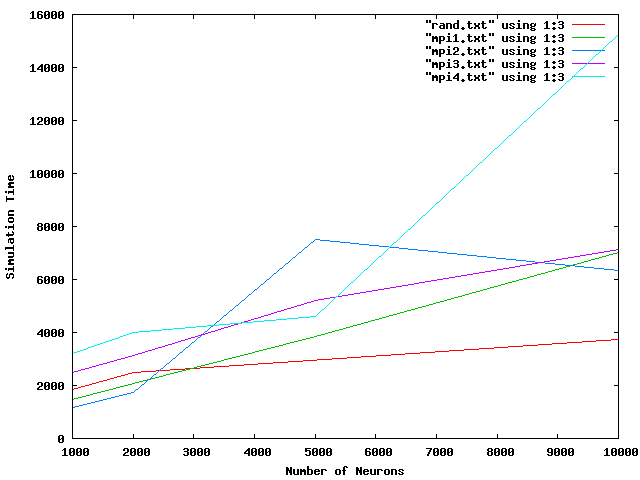
\includegraphics[scale = 0.4]{images/distributed_neurons.png}
\end{center}
\caption{Comparison of setup time to the number of neurons, synapses and processes}
\end{figure}

The set constants: synapses = 1000, steps = 5000.

This comparison graph shows that from the point of performance, the distributed version does not lose much of its potential - the communication overhead does not highly correlate with the number of neurons. Therefore, potentially for a simulation of a much larger scale, the graph for a distributed simulation of 3 processes would go below the original NeMo graph. The reason for this proposition is that as the number of neurons grows the time taken for a simulation step on a single NeMo implementation grows with a factor of this increase. On the other hand, the distributed version has a more fixed value of growth, and at the same time, the local simulations, depending on the number of clusters are much more computationally feasible as opposed to having one big simulation.

\subsection{Number of synapses}

\begin{figure}[h!]
\begin{center}
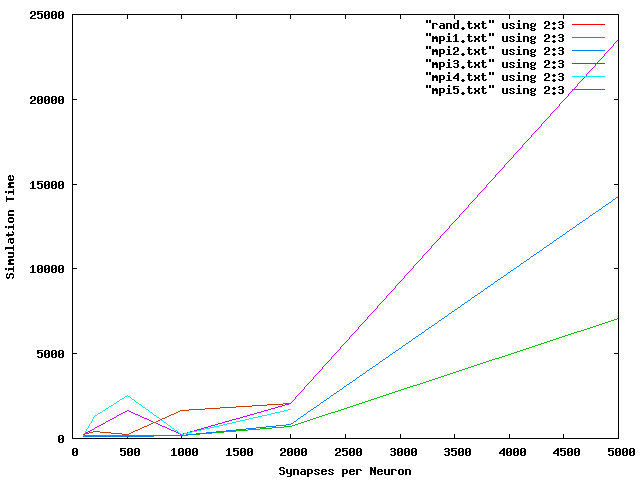
\includegraphics[scale = 0.4]{images/distributed_synapses.png}
\end{center}
\caption{Comparison of setup time to the number of neurons, synapses and processes}
\end{figure}

The set constants: neurons = 2000, steps = 500.

This graph shows that synaptic density per neuron dramatically affects the external spike delivery. Even with the mapping algorithm implemented, the number of spikes fired is still difficult to handle within one simulation step. This particular set of results suggests that there could be much more work done on the inter-nodal communication engine. The graph could also suggest poor choice of constants, as the scope of this simulation is far too small to see the real impact of the distributed simulation. Therefore, potentially, a further set of measurements should be taken to provide a better overall picture.

\subsection{Number of steps}

\begin{figure}[h!]
\begin{center}
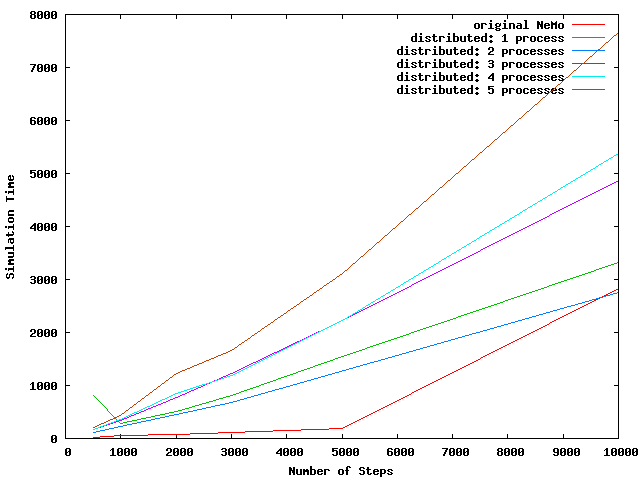
\includegraphics[scale = 0.4]{images/distributed_steps.png}
\end{center}
\caption{Comparison of setup time to the number of neurons, synapses and processes}
\end{figure}

The set constants: neurons = 1000, synapses = 1000.

Through the graph of steps against simulation time it can be easily observed that distributed implementation has a constant per-step time. At the same time the simulation time for the original NeMo simulation went up significantly with the number of steps. This could in turn suggest that as the simulation progresses the number of spikes increases dramatically, causing the decrease in speed of the NeMo simulation. Therefore, if mapping is correctly implemented, as simulation progresses the work that has to be done would be significantly smaller on the sub-simulations, and the external spike delivery will not be ruined by the sudden peaks.

\clearpage

\section{Network throughput during simulation}

\begin{figure}[ht]
\begin{minipage}[b]{0.5\linewidth}
\centering
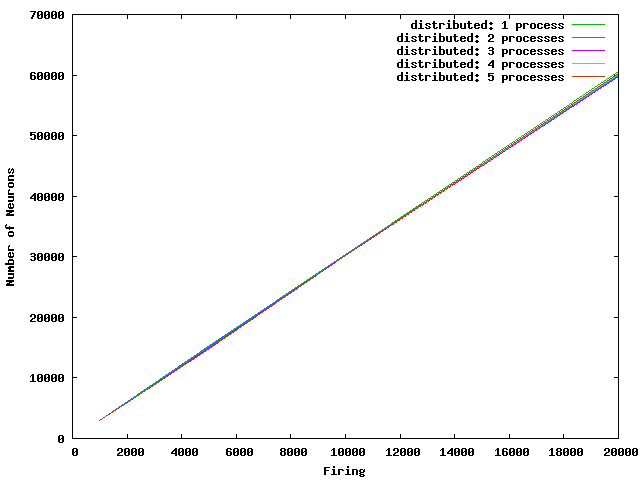
\includegraphics[width=\textwidth]{images/neuron_firing.png}
\caption{Neuron number against firing}
\label{fig:figure1}
\end{minipage}
\begin{minipage}[b]{0.5\linewidth}
\centering
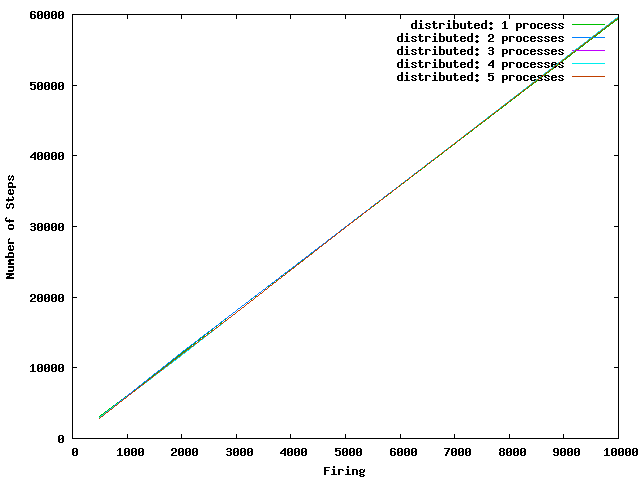
\includegraphics[width=\textwidth]{images/steps_firing.png}
\caption{Number of steps against firing}
\label{fig:figure3}
\end{minipage}
\end{figure}

These two figures show linear proportionality - amount of firing is directly proportional to the number of neurons and number of steps.
The third figure, however, gives a slightly different information. It shows that the synaptic density is not directly proportional to firing capacity.

\begin{figure}[h!]
\begin{center}
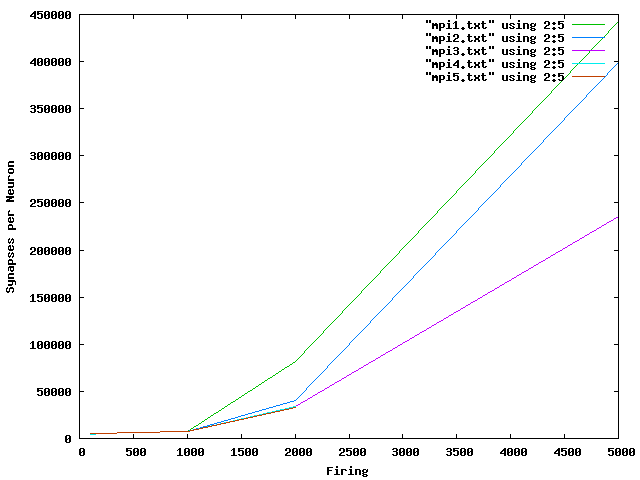
\includegraphics[scale = 0.5]{images/synapses_firing.png}
\end{center}
\caption{Synaptic density against firing}
\end{figure}



